% Self-contained XeLaTeX manuscript. Figures and references are embedded.
% Compile twice with xelatex -no-shell-escape -halt-on-error Out_Execute.tex
\documentclass[11pt,letterpaper]{article}
\usepackage[margin=.88in,headheight=16pt]{geometry}
\usepackage{fontspec}
\setmainfont{lmroman10-regular.otf}[BoldFont=lmroman10-bold.otf,ItalicFont=lmroman10-italic.otf,BoldItalicFont=lmroman10-bolditalic.otf]
\setsansfont{DejaVu Sans}[Scale=.88]
\setmonofont{DejaVu Sans Mono}[Scale=.76]
\newfontfamily\symbolfont{DejaVu Sans}
\usepackage{amsmath,amssymb,amsthm,mathtools,microtype}
\usepackage{booktabs,tabularx,longtable,array,graphicx,xcolor,tikz}
\usetikzlibrary{arrows.meta,positioning,calc,fit}
\usepackage{enumitem,fancyhdr,titlesec,needspace,caption,placeins}
\usepackage[most]{tcolorbox}
\usepackage[round,authoryear]{natbib}
\usepackage{xurl,hyperref}
\definecolor{ink}{HTML}{241A38}
\definecolor{purple}{HTML}{613790}
\definecolor{gold}{HTML}{AA751D}
\definecolor{pale}{HTML}{F5F2FA}
\definecolor{soft}{HTML}{F9F7F2}
\definecolor{muted}{HTML}{686171}
\hypersetup{colorlinks=true,linkcolor=purple,citecolor=purple,urlcolor=purple,
 pdftitle={Out-Execute: Constructing the Conditions of Completion},
 pdfauthor={Vincent Boucher},pdfsubject={Transformational intelligence, executable boundary contracts, semantic containment and persistent outcomes},
 pdfkeywords={Out-Execute, transformational intelligence, completion contracts, incremental computation, compositional execution, SUCCESSOR Omega}}
\urlstyle{same}
\setlength{\parindent}{1.1em}\setlength{\parskip}{.25em}
\setlength{\emergencystretch}{2.4em}\setlength{\tabcolsep}{4.5pt}
\renewcommand{\arraystretch}{1.13}
\widowpenalty=10000\clubpenalty=10000
\setlist{nosep,leftmargin=1.5em,topsep=.35em}
\titleformat{\section}{\large\bfseries\color{ink}}{\thesection}{.65em}{}
\titleformat{\subsection}{\normalsize\bfseries\color{ink}}{\thesubsection}{.65em}{}
\titlespacing*{\section}{0pt}{2.4ex plus .4ex}{1.0ex}
\titlespacing*{\subsection}{0pt}{1.8ex plus .3ex}{.6ex}
\captionsetup{font=small,labelfont=bf}
\pagestyle{fancy}\fancyhf{}
\fancyhead[L]{\small\sffamily OUT-EXECUTE}
\fancyhead[R]{\footnotesize\sffamily TRANSFORMATIONAL INTELLIGENCE}
\fancyfoot[L]{\footnotesize\sffamily Vincent Boucher / MONTREAL.AI}
\fancyfoot[R]{\small\thepage}\renewcommand{\headrulewidth}{.3pt}
\renewcommand{\topfraction}{.94}\renewcommand{\bottomfraction}{.85}
\renewcommand{\textfraction}{.06}\renewcommand{\floatpagefraction}{.82}
\newcolumntype{Y}{>{\raggedright\arraybackslash}X}
\newcolumntype{P}[1]{>{\raggedright\arraybackslash}p{#1}}
\newtheorem{theorem}{Theorem}[section]
\newtheorem{proposition}[theorem]{Proposition}
\newtheorem{corollary}[theorem]{Corollary}
\theoremstyle{definition}\newtheorem{definition}[theorem]{Definition}
\theoremstyle{remark}\newtheorem{remark}[theorem]{Remark}
\newcommand{\Out}{\textsf{Out-Execute}}
\newcommand{\Om}{\texorpdfstring{SUCCESSOR~$\Omega$}{SUCCESSOR Omega}}
\newcommand{\NN}{\mathbb N}\newcommand{\RR}{\mathbb R}
\newcommand{\Dc}{\mathcal D}\newcommand{\Verify}{\mathsf{Verify}}
\newcommand{\dom}{\operatorname{dom}}\newcommand{\supp}{\operatorname{supp}}
\newcommand{\chiG}{\chi}
\newtcolorbox{thesis}{colback=pale,colframe=purple,boxrule=.45pt,arc=1mm,
 left=10pt,right=10pt,top=8pt,bottom=8pt,breakable}
\newcommand{\phead}[1]{\Needspace{4\baselineskip}\paragraph{#1}}
\begin{document}
\thispagestyle{empty}
\begin{center}
{\small\sffamily\color{purple} MONTREAL.AI\quad /\quad TRANSFORMATIONAL INTELLIGENCE $\infty$}\par
\vspace{1.1em}
{\fontsize{42}{47}\selectfont\bfseries\color{ink} Out-Execute {\symbolfont\color{gold}⚡}}\par
\vspace{.6em}
{\Large\bfseries Constructing the Conditions\\of Completion}\par
\vspace{.5em}
{\normalsize From repeated work to reusable means of execution}\par
\vspace{1.1em}
{\large Vincent Boucher}\par
MONTREAL.AI, Montréal, Québec, Canada\par
\vspace{.45em}{\small 21 October 2026\quad /\quad Revised research manuscript}\par
\end{center}
\vspace{.25em}
\begin{abstract}
A completed task can leave an answer, or it can leave a capability that changes what subsequent work must repeat. \emph{Out-Execute} develops the second object. The earlier edition compiled a fixed result's correctness into a region of admissible input changes. Here we go beyond retaining the same answer: construct an executable boundary contract that lets a changed subproblem supply a different answer without re-solving unaffected parts. For finite, separable cost systems, the contract records the exact best completion for every admissible interface assignment. We characterize when two interiors are interchangeable in every external continuation: their complete boundary value functions must agree. This yields an exact stopping rule for propagation, while witnesses and current acceptance still change. An implemented compiler selects boundaries from factor scopes, constructs and independently checks the contracts, repairs changed modules, and assembles a globally optimal artifact. Across 576 synthetic snapshots, all optima agree with full enumeration; 158 updates leave the external contract unchanged. A saved 98-task capability extends to 101 interacting tasks by constructing one new module and retaining 32. A stronger fixed-certificate executor remains competitive and is reported without an invented speedup. Reproduced earlier studies and new local crash/retry tests complete the evidence chain. The contribution is a concrete, testable construction of execution that preserves progress through change, not a new general theory of variable elimination or a claim of autonomous industrial deployment.
\end{abstract}
\begin{thesis}
\centering\large\bfseries
Make progress survive change.\\[.25em]
\normalsize Construct what the next task no longer needs to repeat.
\end{thesis}
\noindent{\small\sffamily THEORY\quad $\cdot$\quad EXECUTED CONSTRUCTIONS\quad $\cdot$\quad REPRODUCIBLE EVIDENCE}
\clearpage

\section{Completion should create a capability}
A requirement changes. A team restarts an optimizer. Another team rebuilds its integration. A third rechecks an unchanged dependency because the handoff contains only a result and a success message. In this hypothetical organization, the bottleneck is not necessarily the intelligence of any participant. It is that completed work has no usable account of what the rest of the organization may safely rely on.

The usual question is \emph{How can we execute this workflow faster?} The transformational question is \emph{What could we construct so that less of the workflow is necessary next time?}

The answer must be stronger than a cache. A changed requirement can genuinely require a new result. It must also be stronger than independent local success: two individually optimal plans can be impossible to combine. A useful completion should therefore leave an executable description of its legitimate interactions, a way to produce the required local response, and evidence that the resulting whole still satisfies the original purpose.

\begin{thesis}
\textbf{Do not merely retain the answer. Retain the means of completing what comes next.}\par\smallskip
A useful execution capability knows what it can preserve, what it must reconstruct, and what it must refuse to claim.
\end{thesis}

This paper builds that object in a precise computational setting. A component retains a table of its best valid completion for each admissible boundary condition. A coordinator combines the tables rather than re-solving every interior. When an interior changes, it is rebuilt and checked locally. If its boundary behavior is unchanged, the change need not propagate through the rest of the optimization---even when the component's actual output has changed. A new receipt still binds the assembled artifact to current input.

The resulting ambition is larger than preserving yesterday's schedule. It is an execution architecture in which an accepted project leaves useful means behind: a qualified interface, constructive responses, validity conditions, complete costs and legitimate reuse rights. Future projects can begin with that capability instead of beginning again.

\subsection{What this revision changes}
\emph{Transformational Intelligence} makes the formulation editable while keeping the authorized purpose as the reference \citep{ti}. \emph{Out-Evolve} directs that freedom toward capabilities that enable later discoveries and constructions \citep{evolve}. \emph{Out-Strategise} asks which capabilities to construct and when to commit to them \citep{strategise}. \emph{Invent the Economy} makes construction, participation, rights, funding and delivery one connected problem \citep{economy}.

The earlier \Out{} manuscript established \emph{fixed-answer persistence}: an optimal schedule and its proof can remain valid on changed inputs \citep{execute1}. Its composition experiment covered disjoint and completely joined task groups. Both results remain useful. Neither supplies a general handoff for interacting components whose internal answers must change.

The new center is \emph{continuation-preserving completion}. It asks what a component must retain so that a future caller can use it under new boundary requirements, and so that replacing its interior does not silently invalidate the rest of the work. This is a more demanding object than one answer, but a much smaller object than repeatedly reconstructing the entire mission.

\subsection{The scientific claim, without a manufactured ranking}
Variable elimination, decomposition, incremental computation and certifying algorithms already provide substantial foundations \citep{dechter,bodlaender,acar,certifying}. The identity underlying our contracts is classical. We do not claim to have invented dynamic programming, nor to outperform every unrestricted implementation of it.

The work developed here is an explicit execution construction: a precise continuation-equivalence boundary; an executable selector for that boundary; independently checked local contracts with witnesses; semantic stopping under changed outputs; a serialized successor with genuine cross-component interactions; and a current-state acceptance service. The new experiments use authored finite models. Their outputs and failures are reproducible. Physical implementation, autonomous invention of primitives and commercial adoption are separate research steps.

\section{Why individually successful work can still fail to complete}
\label{sec:paths}
Consider five unit-duration tasks with pairwise conflicts. There is no capacity limit within a round beyond those conflicts. The required artifact assigns \emph{every} task to the minimum possible number of rounds.

One team handles a path $u-a-v$. A second handles $u-b-c-v$. Each part individually needs two rounds. But the first part's two-round schedules put the shared endpoint tasks $u,v$ in the \emph{same} round, while the second part's two-round schedules put them in \emph{different} rounds. The combined five-cycle requires three rounds. Taking the maximum of the two local optima would return the wrong answer.

\begin{figure}[htbp]\centering
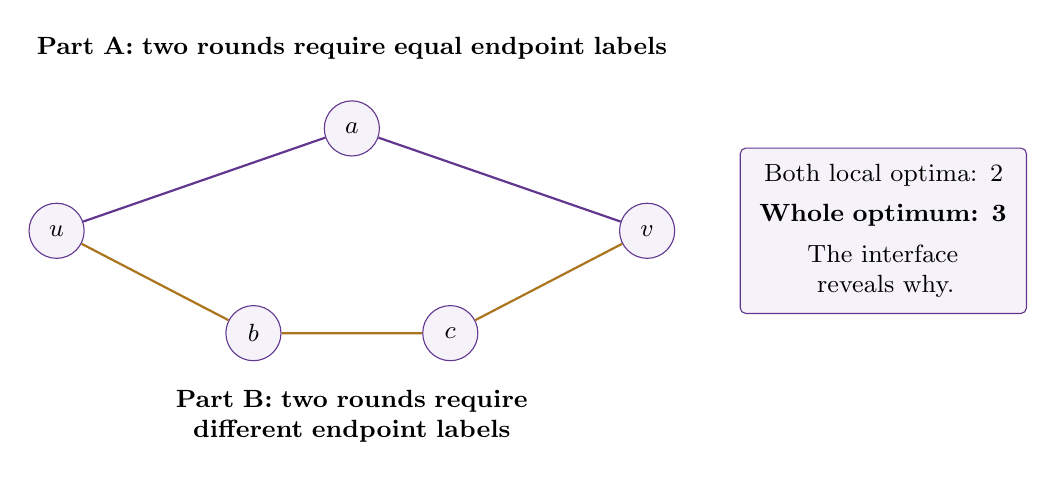
\begin{tikzpicture}[font=\small,>=Latex,
 vertex/.style={circle,draw=purple,fill=pale,minimum size=7mm,inner sep=1pt}]
\node[vertex] (u) at (0,0) {$u$};
\node[vertex] (v) at (7.5,0) {$v$};
\node[vertex] (a) at (3.75,1.3) {$a$};
\node[vertex] (b) at (2.5,-1.3) {$b$};
\node[vertex] (c) at (5,-1.3) {$c$};
\draw[thick,draw=purple] (u)--(a)--(v);
\draw[thick,draw=gold] (u)--(b)--(c)--(v);
\node[above=4mm of a,align=center,text width=8cm] {\textbf{Part A: two rounds require equal endpoint labels}};
\node[below=6mm of $(b)!0.5!(c)$,align=center,text width=8cm] {\textbf{Part B: two rounds require different endpoint labels}};
\node[draw=purple,fill=pale,rounded corners=2pt,align=center,text width=3.4cm,minimum height=2.1cm] at (10.5,0)
{Both local optima: 2\\[.4em]\textbf{Whole optimum: 3}\\[.4em]The interface reveals why.};
\end{tikzpicture}
\caption{Executed exact example. Both parts are correct in isolation; their two-round boundary requirements are incompatible. A constructive interface preserves the information a later composition needs.}
\label{fig:cycle}
\end{figure}

The failure is not fixed by asking either team to repeat its isolated optimization more confidently. It is fixed by changing the \emph{content of the handoff}. Instead of returning only ``two rounds,'' each part returns which boundary assignments can be completed, together with the corresponding local realization. The coordinator then discovers the incompatibility at two rounds and the compatible completion at three.

This distinction applies to the mathematical model, not just its metaphor. Each retained task group can have arbitrary internal conflicts and can interact through the named shared tasks. No conflict is deleted. No task is removed. The constructed interface exposes the exact coupling that the final proof must respect.

\begin{thesis}
\textbf{The output of a subtask should include what makes it usable by another task.}\par\smallskip
A local optimum says how well one part can do. A completion contract says how that part can participate in a correct whole.
\end{thesis}

\section{The executable boundary contract}
\label{sec:model}
\subsection{A finite outcome, not an informal promise}
Let $X$ be finitely many variables with finite nonempty domains. A full assignment $z$ is the requested computational artifact. A finite set of factors describes the authorized constraints and cost:
\begin{equation}
 F_\theta(z)=\sum_{f\in\mathcal F} f_\theta(z|_{\supp(f)}),
 \qquad f_\theta:\dom(\supp(f))\to\NN\cup\{+\infty\}.
 \label{eq:factor}
\end{equation}
Here $+\infty$ means infeasible. Finite costs are nonnegative integers in the implementation. The input $\theta$ includes every factor table, every domain, every scope and the semantic contract. The requirement is to return a feasible assignment attaining the exact minimum, or to establish infeasibility within this finite model. Exhausting a smaller search budget is not such a proof.

Choose boundary variables $B$ and disjoint private groups $X_1,\ldots,X_m$, with $X=B\mathbin{\dot\cup}X_1\mathbin{\dot\cup}\cdots\mathbin{\dot\cup}X_m$. Every factor is assigned exactly once: either wholly to the boundary or to one group and a subset $S_i\subseteq B$. No factor may touch two different private groups. Thus
\begin{equation}
 F_\theta(b,x_1,\ldots,x_m)
 =f_{0,\theta}(b)+\sum_{i=1}^{m}f_{i,\theta}(b|_{S_i},x_i).
 \label{eq:decomp}
\end{equation}
A dependency omitted from this expression invalidates the decomposition. The compiler checks factor ownership from the supplied complete scopes; it does not assume that convenient modularity is a fact about an unobserved physical system.

\begin{definition}[Constructive completion contract]
For module $i$, define its boundary value function and an attaining witness by
\begin{equation}
 v_{i,\theta}(s)=\min_{x_i}f_{i,\theta}(s,x_i),
 \qquad w_{i,\theta}(s)\in\arg\min_{x_i}f_{i,\theta}(s,x_i)
 \label{eq:profile}
\end{equation}
whenever the minimum is finite. The retained contract contains the full domain and table of $v_i$, the witnesses $w_i$, evidence for every finite and infeasible entry, the complete input identity, and the conditions permitting use. It is executable because a valid boundary request selects a concrete local completion.
\end{definition}

A table of favorable examples is not the complete contract. A missing row cannot silently mean infeasible; a claimed minimum requires both an attaining result and a lower-bound justification. In our bounded reference implementation, a separate exhaustive checker establishes each row. Larger systems would need domain-specific proofs or other qualified checking methods.

\begin{theorem}[Exact completion through the boundary]
\label{thm:composition}
Under Equation~\eqref{eq:decomp},
\begin{equation}
 \boxed{\quad \min_z F_\theta(z)
 =\min_{b\in\dom(B)}\left[f_{0,\theta}(b)+\sum_{i=1}^{m}v_{i,\theta}(b|_{S_i})\right].\quad}
 \label{eq:compose}
\end{equation}
If the right side is finite, a minimizing boundary assignment together with each module's attaining witness gives a globally optimal full artifact. If every boundary assignment has infinite cost, the complete problem is infeasible.
\end{theorem}
\begin{proof}
At any fixed $b$, every feasible private assignment costs at least its corresponding $v_i$. Hence the right side is a lower bound on every full assignment. Private groups share no variables once $b$ is fixed, so their independently attaining witnesses can be combined. This attains the lower bound at any finite minimizing $b$. If none is finite, every full assignment violates a factor.
\end{proof}

This is the usual elimination identity \citep{dechter}. Its execution consequence is important: a future external objective or constraint on the same boundary can be evaluated without reconstructing the interiors. The claim remains conditional on the old domains, costs, semantics and allowed attachments. A future requirement about an unexposed private quantity needs an expanded interface.

\subsection{The new object is a family of valid responses}
One stored answer supplies a single assignment. A completion contract supplies a response for every admitted interface condition. The coordinator is free to choose a different boundary condition on a later mission and obtain a different concrete artifact from the same frozen contracts.

This is neither an unlimited catalogue of future tasks nor a claim that every useful problem has a small boundary. Interface size and qualification cost decide whether the construction is worthwhile. The exact profile may be as expensive as the original problem. The benefit is obtained when its scope is useful and its boundary is sufficiently smaller than its interior.

\section{Exactly when an internal change can stop at the boundary}
\label{sec:equivalence}
The first edition asks when an unchanged answer remains correct. The new question is more general: \emph{when can an internal answer change without forcing external optimization to change?}

Consider two versions of a component with the same finite boundary domain and exact value functions $v$ and $v'$. Let an external continuation be any allowed function $h:\dom(B)\to\NN\cup\{+\infty\}$. It represents the remaining constraints and costs after their own private variables have been eliminated. The observer requires both feasibility and the exact optimal value of the assembled problem.

\begin{theorem}[Continuation equivalence]
\label{thm:equivalence}
The following are equivalent:
\begin{enumerate}
\item $v(b)=v'(b)$ for every boundary assignment $b$.
\item For every external continuation $h$, the two assembled problems have the same feasibility and optimal value:
\begin{equation}
 \min_b[h(b)+v(b)]=\min_b[h(b)+v'(b)].
 \label{eq:context}
\end{equation}
\end{enumerate}
In particular, a summary that must support \emph{every} such continuation cannot identify two distinct value functions as interchangeable.
\end{theorem}
\begin{proof}
Pointwise equality makes the objectives identical. Conversely, suppose the profiles differ at $b_*$. Choose a continuation with $h(b_*)=0$ and $h(b)=+\infty$ elsewhere. The two optimal values are $v(b_*)$ and $v'(b_*)$, including the case where exactly one is infeasible. They differ.
\end{proof}

The last statement is a semantic sufficiency and distinguishability result, not a lower bound on file size or a claim that dense tables are always the best representation. A compressed formula may encode the same function. The necessity statement also depends on the admitted external contexts: if a caller can never request $b_*$, the difference there need not matter to that caller. We use the complete boundary domain to make the guarantee explicit.

\subsection{The answer can change while the external contract does not}
The executed three-variable example has $b,x,y\in\{0,1\}$. Initially the first module costs zero when $x=b$ and three otherwise. Its replacement costs zero when $x=1-b$ and three otherwise. The second module costs zero when $y=b$ and two otherwise. The outside cost is one at $b=0$ and four at $b=1$.

Both versions of the first module have boundary values $(0,0)$. Yet the original full optimum $(b,x,y)=(0,0,0)$ is no longer optimal after replacement: it costs four. The repaired optimum is $(0,1,0)$, still costing one.

\begin{table}[htbp]\centering\small
\caption{Actual exact semantic-containment trace. The full optimum remains one, but blindly retaining the old artifact would return a suboptimal result.}
\begin{tabularx}{\linewidth}{@{}Ycc@{}}\toprule
Object & Before the change & After local reconstruction\\\midrule
First module's interface values & $(0,0)$ & $(0,0)$\\
First module's selected private result & $x=0$ & $x=1$\\
Other module's selected result & $y=0$ & $y=0$\\
Selected boundary & $b=0$ & $b=0$\\
Exact accepted total cost & $1$ & $1$\\
Additional boundary minimizations & --- & $0$\\\bottomrule
\end{tabularx}
\label{tab:containment}
\end{table}

The executor compiles and checks the changed module, discovers that its boundary function is unchanged, obtains its new witness, and retains the external decision. Its input identity, local witness identity and current receipt change. This is not a cache hit on the old answer.

\begin{corollary}[Exact semantic stopping]
\label{cor:stop}
Suppose an already checked decomposition receives changes confined to one module's factor values. Domains, scopes, semantics and all outside factors remain fixed. If the rebuilt module has the same boundary value function, every previous minimizing boundary assignment remains minimizing. Replacing only its local witness reconstructs a globally optimal artifact. No new boundary minimization is required. If the profiles differ, universal stopping for all external continuations is not justified.
\end{corollary}
\begin{proof}
Equation~\eqref{eq:compose} has the same boundary objective after equal-profile replacement. A new attaining local witness preserves the assembled objective value. The last assertion follows from Theorem~\ref{thm:equivalence}.
\end{proof}

\begin{thesis}
\textbf{A change should travel only as far as its consequences.}\par\smallskip
Reconstruct the affected interior. Stop propagation only when its complete external meaning is preserved. Renew acceptance even when the outward result is unchanged.
\end{thesis}

\subsection{Why a local optimum is too little information}
Profiles $(0,2)$ and $(2,0)$ have the same isolated minimum, zero. A continuation requiring boundary value zero distinguishes them immediately: the assembled optima are zero and two. Retaining only the scalar optimum erases information essential to future work. The separate test suite executes this control.

Likewise, retaining a profile without its constructive witnesses is insufficient to deliver the artifact. Equal costs do not manufacture the new private assignment. The reference always obtains a current witness and checks the full final assignment; semantic stopping removes an optimization step, not current-output validation.

\section{Construct the interface instead of assuming it}
\label{sec:selection}
A complete handoff is useful only if its boundary is economical. The reference therefore takes the factor scopes as input and searches for a decomposition, rather than requiring the caller to name the preferred modules.

For a proposed boundary $B$, build a graph connecting variables that occur together in a factor. Remove $B$; the remaining connected components are the private groups. Each factor with private variables must belong to exactly one component. All-boundary factors are retained by the coordinator. This construction neither deletes constraints nor invents independence; it derives conditional independence from complete declared scopes.

For any variable set $A$, write $d(A)=\prod_{v\in A}|\dom(v)|$. The bounded selector uses the explicit work proxy
\begin{equation}
 \widehat W_H(B)=\sum_i d(S_i)d(X_i)
 +H\max_i d(S_i)d(X_i)+(H+1)d(B).
 \label{eq:proxy}
\end{equation}
It represents a complete enumeration bound for initial local construction, a worst single-module rebuild over each of $H$ later updates, and one boundary scan per revision. It does \emph{not} count factor evaluation multiplicity, qualification, output materialization, memory, transmission or monetary cost. It is a deterministic design proxy, not a measured total-cost oracle.

The selector enumerates permitted boundary subsets and chooses the minimum proxy, breaking ties by size and variable name. The empty boundary is included: building no decomposition is a genuine alternative. For the 64 finite-cost fixtures, all subsets of size at most two among eight variables are considered, giving 37 candidates each. For the 98-task extension, a deterministic eight-variable scope-degree shortlist is used before exact size-at-most-three selection. That is exact within the shortlist, not a globally optimal separator search.

\subsection{The compiled response is checked, not self-approved}
For every selected module and boundary assignment, the constructor enumerates its private choices with early rejection of violated factors and nonnegative-cost pruning. It records an exact minimum and a tie-broken witness, or infeasibility. A separately written implementation enumerates the full local assignment space using explicit factor lookup tables and checks all rows and witnesses. It does not import the constructor's transitions or branch ordering.

The qualification binds the complete factor tables and domains, not merely their names. A hash is an identity check after the semantic check; it is not proof that a table is correct. If a proposed factor connects two old private groups, the old decomposition fails and must be rebuilt or abandoned. A hidden cross-component edge is not made harmless by a convenient interface label.

\begin{figure}[htbp]\centering
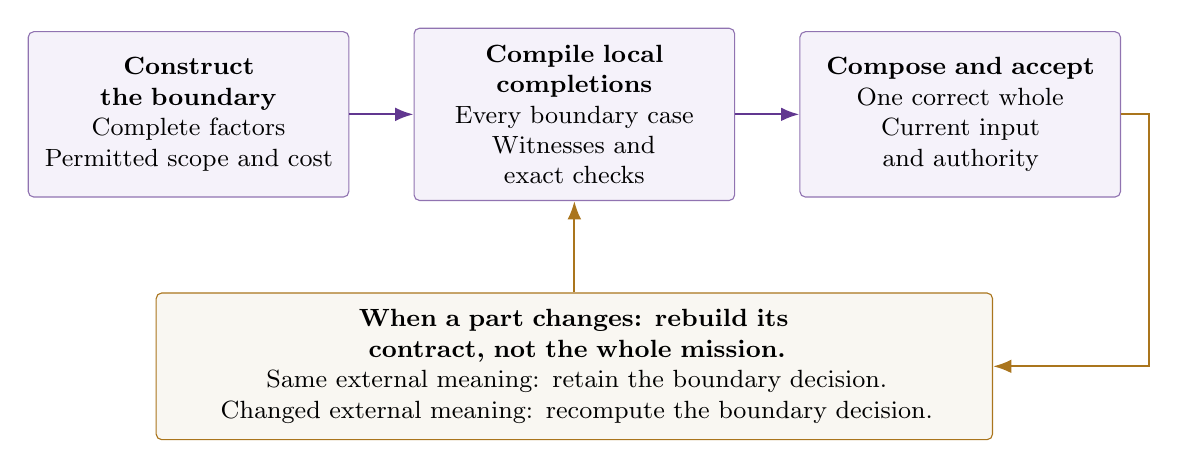
\begin{tikzpicture}[font=\small,>=Latex,
 box/.style={draw=purple!70,rounded corners=2pt,align=center,inner sep=6pt,fill=pale}]
\node[box,text width=3.65cm,minimum height=2.1cm] (a) at (0,0) {\textbf{Construct the boundary}\\Complete factors\\Permitted scope and cost};
\node[box,text width=3.65cm,minimum height=2.1cm] (b) at (4.9,0) {\textbf{Compile local completions}\\Every boundary case\\Witnesses and exact checks};
\node[box,text width=3.65cm,minimum height=2.1cm] (c) at (9.8,0) {\textbf{Compose and accept}\\One correct whole\\Current input and authority};
\draw[->,thick,draw=purple] (a)--(b);\draw[->,thick,draw=purple] (b)--(c);
\node[box,text width=10.2cm,fill=soft,draw=gold] (d) at (4.9,-3.2) {\textbf{When a part changes: rebuild its contract, not the whole mission.}\\Same external meaning: retain the boundary decision.\\Changed external meaning: recompute the boundary decision.};
\draw[->,thick,draw=gold] (c.east)--++(.35,0)|-(d.east);
\draw[->,thick,draw=gold] (d.north)--(b.south);
\end{tikzpicture}
\caption{Implemented construction and update structure. Local qualification and current-state publication remain real work. The circuit does not grant authority to change the required outcome.}
\label{fig:circuit}
\end{figure}

\subsection{A declared limit is better than a disguised assumption}
Large boundaries can make the table exponential. Dense factor scopes can prevent useful separation. Uncertain physical constraints are not made exact by placing them in a finite table. A new objective depending on a hidden private variable can invalidate the old interface. These are reasons to choose another representation, obtain better evidence, retain the original workflow, or decline a claimed guarantee.

The method searches a finite representation grammar. It does not autonomously discover the domain's physical laws, infer missing permissions or establish that a proposed commercial task has a buyer. The broader research target is to discover useful interfaces from natural tasks; this paper constructs one exact mechanism those interfaces can support.

\section{Execution under change: retain, reconstruct, compose, commit}
\label{sec:execution}
There are two complementary forms of retained progress.

\textbf{Fixed-result retention} keeps an artifact and its proof when their input-validity guards still hold. This is the earlier edition's mechanism. \textbf{Continuation-preserving reconstruction} changes an artifact inside a module while keeping its complete interface behavior. The second mechanism is useful precisely when the first may fail.

\begin{table}[htbp]\centering\small
\caption{Different claims require different retained objects. These mechanisms can be combined; a broader contract is not automatically cheaper to construct or check.}
\begin{tabularx}{\linewidth}{@{}P{.21\linewidth}YY@{}}\toprule
Situation & What may be retained & What must still occur\\\midrule
Identical inputs & Exact-input artifact & Identity, authority and current acceptance checks.\\
Changed input, same fixed proof valid & Artifact and proof & Complete guard transport; a new current-input receipt.\\
Changed interior, same boundary function & Outside decision and unaffected modules & Reconstruct and qualify the changed interior; obtain its current witness.\\
Changed boundary function & Unaffected module contracts & Recompute the interface decision and materialize its witnesses.\\
Changed scope, domains or meaning & Only separately requalified assets & Reconstruct the interface or use a qualified fallback.\\\bottomrule
\end{tabularx}
\label{tab:levels}
\end{table}

The new reference compares complete snapshots, identifies changed factors and rebuilds their owning modules. If no all-boundary factor changed and all rebuilt profiles agree pointwise with their predecessors, it retains the selected boundary and refreshes the affected witnesses. Otherwise it scans the boundary objective again. It does not yet maintain a hierarchically indexed incremental minimum or perform distribution-aware scheduling of the contract checks.

Output reconstruction is not free. The reference materializes the full assignment, checks every original factor for feasibility and cost, and produces current identities. A local semantic stop means no new \emph{boundary optimization}; it does not mean no ingestion, checking, copying, hashing or publication work.

A production controller could first try cheap fixed-proof retention and build wider contracts only when a useful reuse horizon justifies them. The package contains both mechanisms, but the two main experimental executors are measured separately. We do not retroactively report an unimplemented hybrid as an observed winner.

\section{Executed evidence: a changed answer, a retained capability}
\label{sec:results}
\subsection{The 576-snapshot finite-cost study}
The principal new study uses 64 separately seeded, authored fixtures. Each has eight ternary variables: two possible boundary variables and three two-variable interiors. Unary and pairwise factor tables contain exact nonnegative costs and forbidden combinations. Complete scopes are supplied; the selector discovers the best boundary in its stated 37-candidate grammar. The subsequent eight revisions per fixture change one table entry at a time without consulting the current solution or contract.

Each of the 576 snapshots is also solved by a separate exhaustive enumeration of all $3^8=6561$ complete assignments. This checks the exact objective independently of the decomposition. Every initial and rebuilt local contract receives the separate full enumeration described above. Every assembled artifact is checked against all original factors.

\begin{table}[htbp]\centering\small
\caption{Actual new finite-cost results. Revisions within a fixture are dependent observations; the fixtures verify a supplied computational model, not the prevalence of useful opportunities in an economy.}
\begin{tabularx}{\linewidth}{@{}Yr@{}}\toprule
Object measured & Result\\\midrule
Seeded fixtures / complete input snapshots & $64\;/\;576$\\
Optima agreeing with full independent enumeration & $576/576$\\
Boundary candidates inspected & $2368$\\
Local contracts constructed, including initial construction & $648$\\
Local constructions if every module were rebuilt at every snapshot & $1728$\\
Updates whose complete external contract is unchanged & $158/512$\\
Updates requiring a new boundary minimization & $354/512$\\
Updates changing the selected full assignment & $60/512$\\
Independent full-problem assignments audited & $3{,}779{,}136$\\
Independent local assignments audited & $52{,}488$\\\bottomrule
\end{tabularx}
\label{tab:finite}
\end{table}

The 648 constructions include 192 initial module builds and 456 affected-module rebuilds. Fifty-six revisions touch only boundary factors. The 158 stops are not a guarantee about a natural workload: they are exact events in the retained generated inputs. The isolated semantic-containment example in Table~\ref{tab:containment} separately demonstrates an unchanged profile with a changed concrete answer; the random bank does not need that curated example to establish its own counts.

The comparison with 1728 full rebuilds isolates reuse. It is not a victory over a strong incremental implementation, which can retain exactly these contracts and make the same decisions. Compiler search, boundary selection, local qualification and full output checks remain in the resource ledger. No wall-clock multiplier, labor saving or energy reduction is inferred from construction counts.

\subsection{A larger task family with real coupling}
A second authored construction has 98 tasks organized through complete declared conflict scopes. The compiler's boundary search selects the round-count variable and two shared task labels. The remaining 96 task variables become 32 three-task modules. Their interactions with both shared tasks remain explicit. This is neither a disjoint union nor a complete join.

The palette is bounded at five. For this generated family that bound is sufficient: the two shared tasks can use different colors, and each three-task interior can use three additional colors. The objective minimizes the shared round-count variable; constraints require every task's label to lie below it and every active conflict's labels to differ. The compiler therefore returns an exact minimum-round schedule for the full family, not merely a feasible five-round schedule.

Across the initial snapshot and sixteen allowed edge changes, the new engine constructs 48 local profiles in total, stops semantic propagation six times and performs eleven boundary reductions. The earlier fixed-certificate executor is run on the same graph sequence and agrees on every optimum. It performs only \emph{two full synthesis calls}, retaining twelve updates and repairing three. This is a strong alternative, not a result to hide. Forty-eight small profile builds and two graph syntheses are different kinds of work; neither count alone ranks the executors.

The new capability's distinctive result is its external scope and constructive composition. It can answer fresh boundary requests, and it can import a new interacting module, rather than relying only on one fixed global schedule or the two old union/join identities.

\subsection{The successor is actually assembled from retained contracts}
The initial 98-task circuit is written to disk, including its full inputs, decomposition, profiles and witnesses. The extension driver reads that file back. It adds a three-task module attached through the same two shared task interfaces, producing a \textbf{101-task} problem. Old factor values and domains are kept exactly; newly admitted factors belong only to the new module and the existing boundary.

\begin{table}[htbp]\centering\small
\caption{Executed interacting successor. The absence of old-module construction does not erase import audits, boundary reduction, current-output checks or the independent full-solve comparison.}
\begin{tabularx}{\linewidth}{@{}Yr@{}}\toprule
Successor quantity & Recorded result\\\midrule
Old tasks / successor tasks & $98\;/\;101$\\
Retained module contracts read from disk & $32$\\
Old module constructions repeated & $0$\\
New module contracts constructed & $1$\\
Fresh full global solve used as an audit & $1$\\
Objective agreement with that audit & Exact\\\bottomrule
\end{tabularx}
\label{tab:successor}
\end{table}

The demonstration deliberately re-audits imported local contracts rather than pretending that file identity proves their truth. That work is recorded. In a maintained trusted qualification store, unchanged certified contracts can be referenced without repeating that import audit, subject to the store and checker assumptions. The experiment does not count that prospective saving as realized.

A separate weighted circuit is also frozen and reopened before 32 new outside objectives and constraints are supplied at its boundary. All 32 assembled optima match fresh full enumeration, with no old module construction. These are different requested continuations inside the same finite mathematical class, not 32 independent businesses or cross-industry physical trials.

\subsection{The earlier results remain intact}
The original package is included unmodified. Its substantive graph, region, composition and system outputs were rerun and matched. The earlier exhaustive block checks $1{,}048{,}576$ certificate--input pairs. Its unfiltered graph bank makes 131 full synthesis calls over 544 snapshots, with 369 retained updates and 44 repairs; the certificate-aware comparator ties its decisions. The original 50 unit-test methods pass again.

Those results support fixed-proof persistence. They are not added to the new fixture count as independent discoveries. The previous browser limitation also remains a limitation: the earlier HTTP study and offline rendering are not relabeled as successful autonomous browser execution in this revision.

\section{A completion must survive delivery, not merely computation}
\label{sec:store}
A correct collection of contracts can still be delivered incorrectly. One module may refer to an old input, one worker may have finished after authority was revoked, or a retry may present an already committed result as a new effect. The current artifact therefore needs a separate acceptance boundary.

The new local service stores immutable specifications, qualified profile records and receipts in SQLite. Qualification runs the independent local checker \emph{before} admitting a profile to the registry. Publication takes a current snapshot, a decomposition, profile identities, an assembled answer and a persistent request identity.

Within one write transaction it checks the current revision and authority, binds every profile to the correct current factor tables and domains, verifies complete factor ownership, recomputes the boundary optimum from the qualified tables, and checks the full returned assignment. It then atomically installs the receipt and the accepted head. An input edit clears current acceptance while leaving historical records intact. Retrying the same bound request returns its existing receipt; rebinding that identity to another payload is rejected.

\begin{proposition}[Publication of a composed completion]
\label{prop:publish}
Assume a correct local qualifier and composition checker, complete controlled input updates, immutable qualified records, faithful identity comparisons and SQLite's stated atomic transaction behavior. Every visible accepted head then names an artifact attaining the required optimum for that head's current specification, installed under authority valid at commit. A replay cannot create a second committed publication for that request. A crash before commit exposes no partial accepted publication; a crash after commit permits recovery of the recorded receipt.
\end{proposition}
\begin{proof}
Qualification establishes the exact local values and witnesses. Publication checks that each qualified record belongs to the current factor partition, so Theorem~\ref{thm:composition} establishes the current global optimum. The full-assignment check establishes attainability. Revision and authority checks occur inside the same serialized write transaction as the receipt and accepted pointer. Input changes clear the pointer atomically. Induction over committed transactions proves the invariant; persistent request binding and transaction atomicity give the replay and crash conclusions.
\end{proof}

The underlying retry and transaction principles are established work \citep{rifl,sqlite}. The new implementation connects them to the composed completion contract. It is not a new distributed consensus algorithm or a proof about arbitrary external browser actions.

\subsection{Actual fault tests}
The new service kills a child process with \texttt{os.\_exit(73)} at six points: before the transaction, after it begins, after the composition check, after receipt insertion, after the head update and after commit. Each store is reopened and the request retried twice. All six runs produce exactly one final accepted receipt, with no partial precommit acceptance. Four separate two-process publication races each produce one commit and one rejected stale contender.

The new 41-method unit suite includes stale profile vectors, changed specifications, false interface summaries, incomplete tables, wrong minima, wrong witnesses, hidden cross-coupling, revoked authority, rebound request identities, stale snapshots and historical replay. All tests pass. The old package's 24 process-crash cases and twelve races were reproduced separately, not merged into these new counts.

\subsection{The boundary of an honest completion claim}
If a remote service may have performed an irreversible action but lost its acknowledgement, a client without a durable request key or a reliable outcome query can be unable to distinguish ``done'' from ``not done.'' Retrying can duplicate the effect; not retrying can omit it. The appropriate transformation is a better action interface, not additional confidence. Our local transaction provides that interface only inside its controlled datastore.

A profile hash also does not authorize access, establish a physical measurement, or detect a falsely declared semantic version. Qualification and publication remain conditional on their actual sources of truth. Safety under the modeled conditions does not guarantee eventual completion under perpetual input changes or permanent failure.

\section{What intelligence should construct next}
\label{sec:program}
The important generalization is not that every task is a graph or a finite table. It is that the \emph{interface between completed work and future work} can itself be an object of invention.

For a natural engineering task, an intelligent constructor could discover a representation with a small sufficient boundary, create an instrument that makes that boundary observable, or redesign a production interface so that independently qualified components really can be composed. Those changes can reduce later search, integration and verification simultaneously. They also incur construction and qualification costs and can fail to preserve the required purpose.

\begin{thesis}
\textbf{The enduring output is not activity. It is a new ability to finish.}\par\smallskip
A completed mission should leave an executable means that another mission can use, challenge, repair and extend.
\end{thesis}

Computer use is a means of reaching existing applications, not a duty to repeat their original click paths. A permitted structured interface can be preferable when it preserves the user's requirements. An interface that removes a required approval or hides a consequential side effect does not. The present experiments contain no frontier-model calls and do not measure how often an autonomous agent discovers such a transformation.

A civilization of agents would need more than shared conversation history. It would need interoperable capabilities with meaningful scope, current evidence and legitimate authority. The finite contracts here illustrate one exact way that independently completed work can become usable by another project. Extending the idea to scientific instruments, industrial systems and energy infrastructure requires domain-specific constructions, not relabeling finite optimization as physical production.

\section{SUCCESSOR \texorpdfstring{$\Omega$}{Omega}: make preserved progress valuable}
\label{sec:business}
The proposed commercial object is a \emph{maintained completion capability}: an agreed route from changing, authorized requirements to accepted current artifacts, with explicit update scope, rejection rules, recovery behavior, service obligations and reuse rights. It can be sold through funded construction, qualified integration, accepted deliverables or genuine ongoing support.

This makes \emph{Invent the Economy} part of the technical mechanism \citep{economy}. The buyer's acceptance criteria define what the boundary must preserve. Permission to deliver any optimal assignment, instead of repeating a prescribed solver, creates the room for a different execution architecture. An accepted component interface can let several applications share construction. Reuse rights determine which subsequent callers may use it. Cash timing determines whether the capability can be built before later receipts arrive.

The provider should benefit from eliminating unnecessary execution, rather than require extra agent activity to preserve revenue. Compensation can attach to dependable accepted capability. Competitive prices and genuine demand still matter: a mature incremental system may already supply the same benefit.

For a horizon of $T$ revisions, compare complete campaigns, not only application calls:
\begin{equation}
\begin{aligned}
 C_{\mathrm{life}}={}&C_{\mathrm{discover}}+C_{\mathrm{construct}}+C_{\mathrm{qualify}}+C_{\mathrm{integrate}}\\
 &+\sum_{t=1}^{T}\big(C_{\mathrm{ingest},t}+C_{\mathrm{local},t}
 +C_{\mathrm{compose},t}+C_{\mathrm{check},t}+C_{\mathrm{publish},t}\big)\\
 &+C_{\mathrm{maintain}}+C_{\mathrm{remedy}}+C_{\mathrm{finance}}.
\end{aligned}
\label{eq:life}
\end{equation}
Failed constructions, discarded profiles, human expertise and independent review remain charged. Saved optimization calls do not by themselves establish lower total cost. Unrestricted opening cash plus receipts actually usable by each date must cover incurred expenditure, continuing obligations and protected reserves. A future acceptance invoice is not present construction money.

The retained business asset is a qualified compiler and implementation, valid deployment rights, compatible interfaces, maintained evidence and actual customer relationships. Public algorithms do not become exclusive property because a company uses them. MONTREAL.AI's parent ownership remains intact; any separately financed venture or asset agreement requires its own negotiated terms. The AGIJobManager USDC route and Alpha / Jobs v0 \$AGIALPHA routes remain distinct, with no new token-holder entitlement implied.

Alpha can investigate and construct the missing interface; Jobs can commission bounded implementation and evaluation; Fleet can supply qualified execution within its configured authority. These are intended architectural roles, not a claim that this research implementation is already deployed in the four repositories.

\begin{center}
\textbf{Find your Alpha. Build your SUCCESSOR $\Omega$.}\par\smallskip
\url{https://github.com/MontrealAI/AGI-Alpha-Agent-v0}
\end{center}

The long-term ambition is an accumulating ability to deliver more demanding science and productive capacity. Accepted work can leave reusable methods, instruments and earned resources after obligations. Those assets can support a different successor. Every link still requires technical validity, useful demand and actual resources. A compiled schedule is not a commissioned laboratory, and a large possible-input count is not a valuation.

\section{Closest prior work and the experiment that would matter next}
\label{sec:related}
\phead{Elimination and interface state.}
Bucket elimination and tree-decomposition methods already retain functions over small boundaries to solve larger structured problems \citep{dechter,bodlaender}. Our Equation~\eqref{eq:compose} belongs to that tradition. The continuation-equivalence argument states precisely what a reusable value interface preserves for the declared class of external continuations; it is not a claim to priority over contextual equivalence or finite-state reasoning. The new code makes this boundary a checked execution artifact with constructive witnesses, replacement and current-state publication.

\phead{Incremental computation and stopping.}
Self-adjusting computation establishes consistency between change propagation and from-scratch evaluation \citep{acar}. Build-system research makes rebuilding policies explicit and executable \citep{build}. A sufficiently capable incremental system can implement our contracts and the same semantic stopping. Our purpose is to construct the qualified intermediate object, not to deny these precedents or to treat their omission as an experimental advantage.

\phead{Certificates and operational acceptance.}
Certifying algorithms separate a result producer from a checker \citep{certifying}. Reliable retry infrastructure and SQLite's transaction semantics supply the operational foundations \citep{rifl,sqlite}. The retained original region compiler and the new contract publisher combine these ingredients at different levels. Their checkers share authorship with the research; they are distinct implementations, not external institutional review.

\phead{The next claim must be earned on natural work.}
A decisive follow-on would commission independently selected changing workloads whose outcomes matter to an actual user. Give a model-assisted constructor, a domain specialist and modern incremental systems the same initial information, legitimate tools, time, authority and full resource budget. Allow every competitor to redesign the decomposition and use proof-aware reuse. Freeze the constructed interface before revealing fresh external objectives and a successor attachment. Measure accepted outcomes, full cost, recovery, false acceptance, rejected invalid scope and the value of inherited assets.

The present study does not establish superiority in that campaign. Its contribution is a finished mechanism, proofs and executable evidence that make such a campaign possible to specify and refute. The old graph-aware executor's strong showing is a useful constraint on the ambition: an unnecessarily broad contract can cost more than a sufficient fixed proof.

\section{Conclusion: construct what the next task no longer needs to repeat}
An answer can be correct and still be a poor inheritance. It may omit how it can participate in a larger outcome, what input changes it tolerates, or how its acceptance can be renewed after interruption. Repeating the answer-producing process does not repair the missing interface.

\Out{} makes completion a construction target. A fixed proof can preserve one result across many changed inputs. An executable boundary contract can preserve an entire external decision problem while its internal result changes. Checked composition can turn retained modules into a larger interacting capability. Current-state publication ensures that these mathematical relationships produce an accepted artifact rather than a stale success message.

The technical result is exact within the stated finite model. The larger research challenge is to discover which interfaces, instruments and productive structures make that kind of inheritance useful in the world. That is the point at which transformational intelligence becomes an execution advantage: not because it performs more activity, but because it constructs better conditions for dependable completion.

\begin{thesis}
\centering\large\bfseries
Make progress survive change.\\[.25em]
\normalsize Leave the next project with less to reconstruct\\and more that it can legitimately accomplish.
\end{thesis}

\section*{Evidence status}
This AI-assisted manuscript contains written proofs, exact finite computations, actual local process/database tests and proposed scientific and commercial applications. It does not report physical experiments, a controlled frontier-agent invention campaign, external peer review, customer contracts or realized revenue. No repository, operational system, wallet or permission was changed. The original paper and its package are preserved unmodified.

\clearpage\appendix
\section{The preserved fixed-certificate result}
\label{app:old}
For a graph $G=(V,E)$ with fixed labeled tasks, let $s$ be a total $k$-round coloring. Its lower-bound proof $\pi$ is either a $k$-clique or a complete canonical refutation of $(k-1)$-colorability. Structural proof checks are independent of the graph edges; the refutation's input-dependent leaves cite positive conflict edges. Write
\begin{equation}
 E^-(s)=\{\{u,v\}:s(u)=s(v)\},\qquad E^+(\pi)=\{\text{edges explicitly required by the lower proof}\}.
\end{equation}
The fixed certificate is accepted exactly on
\begin{equation}
 \Dc(s,\pi)=\{E:E^+(\pi)\subseteq E,\ E\cap E^-(s)=\varnothing\}.
 \label{eq:oldregion}
\end{equation}
A proper coloring gives the upper bound $k$; the surviving proof gives the lower bound $k$. Conversely, a missing positive literal or a present negative literal fails the fixed checker. If the region is nonempty, its literals are disjoint and
\begin{equation}
 |\Dc(s,\pi)|=2^{\binom{|V|}{2}-|E^+(\pi)|-|E^-(s)|}.
\end{equation}
Every literal is necessary for acceptance of this fixed proof. This is not the largest semantic correctness region over all possible alternate proofs.

A complete authoritative edit mask identifies which literal predicates need re-evaluation. This proves residual guard transport when the artifact, proof and semantic contract are unchanged. A partial edit feed or an unreported semantic amendment invalidates the claim. The original executor compares the actual old and new graph snapshots instead of trusting an unverified mask.

The old persistence-design example considers twenty vertices with one triangle. Optimal three-round assignments of sizes $(18,1,1)$ and $(7,7,6)$ require 153 and 57 negative edge literals respectively, plus the same three positive clique edges. Their exact fixed-certificate regions have sizes $2^{34}$ and $2^{130}$. These are input-class cardinalities, not measured speedups. The strongest certificate-aware baseline in the original study makes the same retention decisions as the region compiler.

The original complete package contains the explicit refutation language, its symmetry-reduction proof, bounded repairs, exhaustive verification, all input streams and the original publication implementation. It remains the source for those definitions and is included byte-for-byte. Reproduction of its calculations does not turn its synthetic evidence into physical evidence.

\section{Contracts, proof obligations and complete scopes}
\label{app:proofs}
\subsection{Why a boundary contract is sufficient}
Let all private domains be finite. For a fixed boundary assignment $b$, the feasible private choices form a Cartesian product because no factor touches two private groups. The infimum of the sum is therefore the sum of the attained local minima, with $+\infty$ propagating infeasibility. Minimizing over $b$ proves Equation~\eqref{eq:compose}. If an outside constraint touches an unexposed private variable, the product argument is no longer valid. The compiler checks complete factor ownership before applying it.

The constructive witness is essential. For each finite row, the checker requires an assignment to every private variable and independently verifies its domain, factor feasibility and exact cost. For optimality, it also enumerates all other private assignments and excludes a cheaper one. For an infinite row, it confirms that no feasible assignment exists. This exhaustive reference is intentionally bounded; no universal claim of inexpensive checking is made.

\subsection{What the continuation theorem does not say}
Theorem~\ref{thm:equivalence} preserves feasibility and optimal value under every admitted outside continuation. It does not preserve a particular private assignment or every optimum's identity. A new private witness can be required, as Table~\ref{tab:containment} demonstrates. It also does not preserve a secondary preference that is absent from the cost contract. Adding such a preference requires encoding it before the comparison or making a separately authorized change.

If the required output were only the identity of an optimizer rather than its value, adding the same constant to every finite local value could be unobservable in some contexts. If the boundary is restricted, some profile entries could be irrelevant. Those are different purpose contracts. Our result states the stronger, explicitly named observation: exact cost and feasibility over the complete admitted interface domain.

The pinning continuation used for necessity is available in the mathematical context class, not assumed physically free. A narrower operational class can have a coarser equivalence relation. The current implementation chooses a full finite contract so that its transfer claim is inspectable without an unmodeled caller restriction.

\subsection{The cost of the representation}
For local module $i$, dense storage contains $d(S_i)$ cost entries and at most that many private witnesses. The reference full-enumeration checker evaluates $d(S_i)d(X_i)$ assignments. The constructor can do less through constraint and cost pruning, but this does not change the exponential worst case.

A complete boundary recomposition scans $d(B)$ assignments and consults every module's projected entry plus every boundary-only factor. Full artifact construction and direct feasibility checking depend on the whole output size and factor list. Thus a small boundary removes particular search work; it does not imply constant-time end-to-end execution.

The selector's Equation~\eqref{eq:proxy} prices complete assignment enumeration only. It can be wrong about realized runtime or qualification cost. A production selector needs measured workload distributions, representation alternatives, memory limits and an agreed cost vector. The exact mathematics does not supply those empirical inputs.

\section{The precise implemented input families}
\label{app:fixtures}
\subsection{Finite weighted completion}
The 64 primary seeds are 310000--310063. Variables are $b_0,b_1$ and $m_ix_j$ for $i\in\{0,1,2\}$ and $j\in\{0,1\}$, all with domain $\{0,1,2\}$. Every variable has a unary table. Pair tables connect the two boundary candidates, each private pair, and each private variable to both boundary candidates. These complete possible scopes remain fixed during the stream.

Unary costs are independent seeded integer draws in $\{0,\ldots,5\}$. Each pair-table entry is forbidden with probability 0.10 under the specified pseudorandom generator, otherwise an integer in $\{0,\ldots,4\}$. Eight subsequent updates use a separate generator seeded at the fixture seed plus 1000000. An update uniformly chooses a factor and an entry, then assigns a different value from $\{+\infty,0,1,2,3,4,5\}$. The full realized tables, not only the seeds, are saved.

Every boundary subset of size at most two is scored with $H=8$. In the recorded fixtures the selected boundary is the two shared variables and there are three private modules. The choice follows from the complete supplied scopes and the stated proxy; it is not an autonomous discovery of a natural scientific law. Revisions are not selected according to whether they help the new executor.

The independent optimum checker enumerates every full assignment at every revision. The local checker uses explicit Python dictionaries rather than the constructor's flattened table indexing and search order. Source hashes, counters, selected boundaries, all snapshots, answers and final contracts are retained. Shared authoring means the two implementations are not institutionally independent.

\subsection{Graph construction and a truly interacting successor}
For the larger study, tasks 0 and 1 are shared. Group $i$ contains tasks $2+3i,3+3i,4+3i$, for $i=0,\ldots,31$. Possible pairwise conflicts are every pair within the shared tasks plus one private group. The seed 320000 activates each possible conflict independently at probability 0.45. Sixteen revisions, seeded at 320001, toggle a uniformly selected allowed edge, without using the current certificate.

The finite optimization has one variable $K\in\{1,\ldots,5\}$ and a color variable in $\{0,\ldots,4\}$ for every task. Unary cost $K$ is charged once. Palette constraints require $c_v<K$. Active conflicts require unequal endpoint labels; inactive conflicts have zero cost at every pair but keep their declared possible scope. The scope graph thus represents the allowed mutation family, not a claim that an inactive constraint currently binds.

Boundary selection first takes the eight variables with highest factor-scope degree, breaking ties by name, and enumerates all subsets up to size three within them: 93 candidates. It selects $K$ and the two shared task labels. This limited candidate grammar is stated rather than presented as a complete search over all 99 variables.

The 101-task successor preserves all original factors and their values, and adds one further three-task group's factors. Its old private groups remain untouched. The actual retained JSON file is loaded before construction. Every imported profile is checked again in this experiment; those audits are included. A fresh global graph solve independently matches the final objective and is counted as an audit, not concealed as part of a supposedly solve-free execution.

\subsection{Fresh external continuations}
The weighted continuation study freezes a separate problem at seed 330000 with the same interface structure. It saves and reopens its profiles, then supplies 32 new sets of boundary-only tables using seed 330001. Each new entry is infeasible with probability 0.15, otherwise an integer in $\{0,\ldots,7\}$. Interior tables remain fixed. Full enumeration independently verifies all 32 results. The experiment tests the declared continuation scope; it is not transfer to unrelated physics or customer preferences.

\section{Storage, qualification and current-state safety}
\label{app:storage}
The new database contains four types of record: the current head, immutable specifications indexed by revision, immutable qualified profiles indexed by content identity, and receipts indexed by both request and revision. Profile qualification is separate from publication. The qualifier checks every row, including the consistency of the serialized semantic summary with its actual entries. An unverified summary cannot suppress propagation merely by claiming equality.

Publication rechecks current state inside \texttt{BEGIN IMMEDIATE}. The profile vector must be complete and aligned with the decomposition. Every original factor appears exactly once. Each profile's private variables, boundary variables, domain values, semantics and tables must match its assigned current module. The coordinator's finite reduction establishes the lower bound; the complete returned assignment attains it. A changed input, changed authority, mismatched profile or wrong objective prevents a new accepted head.

Qualified profiles may remain in the registry after a failed or stale publication. That preserves useful work without treating it as current acceptance. A later revision can reuse one only if its complete input binding still matches. Historical retries return history and do not set the current accepted pointer. A revoked authority blocks new commits but does not rewrite the fact that an earlier authorized publication occurred.

The store owner, file integrity, correct semantic declarations, Python implementation and SQLite transaction behavior are inside the stated trust boundary. The tests do not cover malicious database administrators, storage corruption, power loss, side-channel attacks, distributed consensus or remote irreversible effects. Hard process termination is stronger than a caught exception, but it is not every possible failure mode.

\section{Reproducibility and changes during development}
\label{app:reproduce}
The new constructor, independent oracle and local publisher use Python's standard library. The recorded interpreter is Python 3.13.5. The full primary run includes boundary search, construction, exhaustive audits, checks and serialization. Its timing is an environment-specific record, not a production performance claim. The old package retains its own timestamps, runtime and browser limitation.

Four separate development seeds, 300000--300003, were used before the primary seed block. The initial attempt to run the full primary block was interrupted by the foreground execution time limit. No selection rule or data generator was changed in response; the complete run was performed in a persistent local process. The interruption and initial protocol are retained. Later hardening made the independent checker reject malformed semantic summaries and interface bindings. The valid study outputs were rerun under the final checker, and the substantive results remained unchanged. This is a disclosed local development history, not external preregistration.

\begin{verbatim}
python reproduce.py --out /path/to/fresh_results
python -m unittest discover -s tests -v
xelatex -no-shell-escape -interaction=nonstopmode \
  -halt-on-error Out_Execute.tex
xelatex -no-shell-escape -interaction=nonstopmode \
  -halt-on-error Out_Execute.tex
\end{verbatim}

The source is self-contained: all figures and the bibliography are embedded. Ordinary installed Latin Modern and DejaVu fonts are used; font binaries are not distributed. The complete earlier package is included unchanged for provenance and reproduction, not silently rewritten into the new experiment.

\begingroup\small
\begin{longtable}{@{}P{.43\linewidth}P{.52\linewidth}@{}}
\caption{Primary new artifacts. Stored outputs are actual executed records. Proposed natural and commercial studies are identified as proposed.}\\
\toprule File & Purpose\\\midrule\endfirsthead
\toprule File & Purpose\\\midrule\endhead

\texttt{code/contracts.py} & Exact boundary selector, compiler, composer, semantic stopping and checked-input restore.\\
\texttt{code/independent.py} & Separately implemented local/global enumeration and composition checks.\\
\texttt{code/fixtures.py} & Complete weighted and graph input generators.\\
\texttt{code/store.py}, \texttt{run\_storage.py} & Qualified-profile registry, current-state commit and actual crash/race tests.\\
\texttt{results/streams.json} & Every primary input revision, selected boundary, returned answer and update decision.\\
\texttt{results/semantic\_containment.json} & Changed private answer with an unchanged external contract.\\
\texttt{results/interacting\_modules.json} & The two individually bipartite paths whose union needs three colors.\\
\texttt{results/retained\_circuit.json} & Actual saved 98-task construction used by the successor.\\
\texttt{results/successor.json} & 101-task outcome, all retained profiles and fresh audit solve.\\
\texttt{results/fresh\_continuations.json} & All 32 new boundary objectives and constraints.\\
\texttt{results/circuit\_storage.json} & Actual six crash cuts and four concurrent-publication races.\\
\texttt{inherited/} & Unmodified original paper/package and new reproduction evidence.\\\bottomrule
\end{longtable}
\endgroup

\FloatBarrier
\section{Skeptical review and the limits that remain}
\label{app:review}
\phead{Is this only ordinary decomposition?}
The mathematical elimination operation is ordinary decomposition and is credited. The contribution is the complete qualified execution object, its precise continuation claim, its semantic replacement rule and the executed integration. A specialist can implement the same mechanism. The paper does not infer discovery-policy superiority from its branding.

\phead{Was independence handed to the algorithm?}
Complete factor scopes and an authored structured family were supplied. The selector computes a boundary from those scopes; it is not given the winning variable names in the primary block. The larger block uses an explicitly limited shortlist. Finding or physically constructing such useful structure in unfamiliar natural work remains untested.

\phead{Can an unchanged profile justify an unchanged artifact?}
No. The old witness may fail or become suboptimal. The reference reconstructs the changed local witness even when it retains the external decision. The small example changes $x=0$ to $x=1$ while preserving the interface values and global optimum. A current full assignment and receipt are still required.

\phead{Is the contract verifier cheap?}
Not necessarily. This implementation enumerates each local finite space to qualify it. The primary study records 52,488 such local audit assignments, plus 3,779,136 independent global audit assignments. The latter are experimental validation, not the work a maintained executor must repeat. Both remain in the full research account.

\phead{Does the new mechanism beat the old executor?}
No universal win is established. On the 98-task stream the earlier fixed-certificate executor needs only two global synthesis calls. The broader profile construction performs different, sometimes unnecessary work. The new scope is exact replacement and arbitrary admitted boundary continuations, not a retrospective victory on a favorable timing ratio.

\phead{Are local proof and authorization interchangeable?}
No. A qualified profile certifies a mathematical relation. The publisher checks the current specification, factor ownership and authority. A valid artifact can still be unauthorized or stale. A successful publication can still rely on an incorrectly modeled physical requirement. These are different checks.

\phead{Does retaining more mean intelligence has improved?}
No. A richer starting capability can improve a later mission without changing the method that discovers capabilities. The successor demonstrates constructive inheritance within one class. A discovery-policy claim requires independently initialized natural campaigns with comparable starting resources and unrestricted competitors.

\phead{What does the revision enable that the earlier paper did not?}
It constructs a complete interface for \emph{different} valid local outcomes, not just a region preserving one fixed outcome. It can requalify a changed interior, keep the unchanged external optimization, and compose a larger mission with partial coupling through named boundary variables. The earlier disjoint/complete-join operators and fixed-result guards alone do not supply that interface. This is the concrete added capability; it is not a claim to have invented the underlying elimination mathematics.

\section{Claim--evidence register and source identities}
\label{app:claims}
\begingroup\small
\begin{longtable}{@{}P{.28\linewidth}P{.33\linewidth}P{.32\linewidth}@{}}\toprule
Claim & Evidence & Scope\\\midrule\endfirsthead
\toprule Claim & Evidence & Scope\\\midrule\endhead
Exact global completion from local contracts & Theorem~\ref{thm:composition}; finite implementation & Complete finite factorization; established elimination identity.\\[3pt]
Exact equivalence under every continuation & Theorem~\ref{thm:equivalence}; pinning counterexample & Feasibility and optimal value; full boundary domain and admitted pinning contexts.\\[3pt]
Changed answer, unchanged exterior decision & Corollary~\ref{cor:stop}; executed three-variable trace & New local witness and current validation remain necessary.\\[3pt]
576 independently checked snapshot optima & Full saved inputs; separate exhaustive oracle & Authored finite model; not a natural workload or autonomous invention study.\\[3pt]
158 semantic propagation stops & Exact update records & Frequency in these 512 revisions only.\\[3pt]
32 fresh outside continuations & Frozen contracts reopened; full oracle comparisons & Boundary-only changes in the same mathematical class.\\[3pt]
98-to-101-task interacting successor & Saved/reopened construction; one new module; global audit & Old modules re-audited; no physical task execution.\\[3pt]
Current local publication survives process interruption & Proposition~\ref{prop:publish}; six crashes and four races & Local controlled SQLite boundary and stated implementation assumptions.\\[3pt]
Earlier results preserved and reproduced & Original archive; new substantive-output comparison; 50 old tests & Earlier synthetic scope and browser limitation unchanged.\\[3pt]
Commercial completion service & Proposed architecture and full-cost account & No customer terms, revenue or token valuation established.\\\bottomrule
\end{longtable}
\endgroup

The exact source basis is the supplied 21-page original \emph{Out-Execute}, the 25-page refined \emph{Out-Strategise}, and the retained foundation versions identified in the original companion: \emph{Transformational Intelligence} (24 pages), \emph{Invent the Economy} (22 pages) and revised \emph{Out-Evolve} (29 pages). The original Out-Execute LaTeX was read in full. Local hashes identify the files retained and used; they are not assertions about all later repository versions.

Outside-source inspection was performed on 21 October 2026 and is recorded separately. Publisher records, author-affiliated records and official documentation support the cited prior-art descriptions. The review is focused, not exhaustive. No live platform status, current model ranking or unsupported automation-market estimate is used as a premise.

\clearpage
\begin{thebibliography}{99}
\small\raggedright\setlength{\itemsep}{.4em}
\bibitem[Boucher(2026a)]{ti}
Vincent Boucher. \emph{Transformational Intelligence: Learning to Change the Game}. MONTREAL.AI, October 2026. Supplied 24-page research manuscript. \url{https://github.com/MontrealAI/AGI-Alpha-Agent-v0/blob/main/docs/Transformational_Intelligence.pdf}.
\bibitem[Boucher(2026b)]{economy}
Vincent Boucher. \emph{Invent the Economy: Transformational Intelligence for Creating Viable Markets}. MONTREAL.AI, October 2026. Supplied 22-page research manuscript. \url{https://github.com/MontrealAI/AGI-Alpha-Agent-v0/blob/main/docs/Invent_the_Economy.pdf}.
\bibitem[Boucher(2026c)]{evolve}
Vincent Boucher. \emph{Out-Evolve: Building the Means of Discovery and Production}. MONTREAL.AI, 20 October 2026. Retained revised 29-page version. \url{https://github.com/MontrealAI/AGI-Alpha-Agent-v0/blob/main/docs/Out_Evolve.pdf}.
\bibitem[Boucher(2026d)]{strategise}
Vincent Boucher. \emph{Out-Strategise: Constructing the Options That Change the Game}. MONTREAL.AI, refined 25-page manuscript, 20 October 2026. Exact supplied PDF and LaTeX identified in the retained companion.
\bibitem[Boucher(2026e)]{execute1}
Vincent Boucher. \emph{Out-Execute: Transformational Intelligence for Persistent Outcomes}. MONTREAL.AI, original 21-page manuscript, 21 October 2026. Original PDF, LaTeX, executable study and results preserved unmodified in this revision's companion archive.
\bibitem[Dechter(1999)]{dechter}
Rina Dechter. Bucket elimination: A unifying framework for reasoning. \emph{Artificial Intelligence}, 113(1--2):41--85, 1999. \url{https://doi.org/10.1016/S0004-3702(99)00059-4}.
\bibitem[Bodlaender(1987)]{bodlaender}
Hans L. Bodlaender. \emph{Dynamic Programming on Graphs with Bounded Treewidth}. MIT Laboratory for Computer Science Technical Report MIT-LCS-TR-394, June 1987. Author-affiliated archive: \url{https://hdl.handle.net/1721.1/149658}.
\bibitem[Acar et~al.(2013)]{acar}
Umut A. Acar, Matthias Blume and Jacob Donham. A consistent semantics of self-adjusting computation. \emph{Journal of Functional Programming}, 23(3):249--292, 2013. \url{https://doi.org/10.1017/S0956796813000099}. Open manuscript: \url{https://arxiv.org/abs/1106.0478}. Cited for the established consistency and change-propagation framework, not as an implementation benchmark performed here.
\bibitem[Mokhov et~al.(2018)]{build}
Andrey Mokhov, Neil Mitchell and Simon Peyton Jones. Build systems à la carte. \emph{Proceedings of the ACM on Programming Languages}, 2(ICFP), 2018. \url{https://doi.org/10.1145/3236774}. Author page: \url{https://simon.peytonjones.org/build-systems-a-la-carte/}.
\bibitem[McConnell et~al.(2011)]{certifying}
R. M. McConnell, K. Mehlhorn, S. Näher and P. Schweitzer. Certifying algorithms. \emph{Computer Science Review}, 5(2):119--161, 2011. \url{https://doi.org/10.1016/j.cosrev.2010.09.009}.
\bibitem[Lee et~al.(2015)]{rifl}
Collin Lee, Seo Jin Park, Ankita Kejriwal, Satoshi Matsushita and John Ousterhout. Implementing Linearizability at Large Scale and Low Latency. \emph{SOSP}, pp.~71--86, 2015. \url{https://doi.org/10.1145/2815400.2815416}. Author project: \url{https://seojinpark.net/projects/rifl/}.
\bibitem[SQLite(2026)]{sqlite}
SQLite. \emph{Transaction}. Official documentation, inspected 21 October 2026. \url{https://sqlite.org/lang_transaction.html}. The linked runtime version is recorded by each executed system study.
\end{thebibliography}
\end{document}
